\documentclass{m2pi}
% %%%%%%%%%%%%%%%%%%%%%%%%%%%%%%%%%%%%%%%%%%%%%%%%%%%%%%%%%%%%%%%%%%%%%%
%                          STANDARD PACKAGES                         %
%%%%%%%%%%%%%%%%%%%%%%%%%%%%%%%%%%%%%%%%%%%%%%%%%%%%%%%%%%%%%%%%%%%%%%

\usepackage{graphicx}
\graphicspath{{figures/}}

\usepackage{epstopdf}
\usepackage{amsthm}
\usepackage{amsmath}
\usepackage{amssymb}
\usepackage{amsxtra}
\usepackage{amscd}
\usepackage{verbatim}
\usepackage{rotating}
\usepackage{multirow}
\usepackage{multicol}
\usepackage{url}
\usepackage[margin=1.5in]{geometry}
\usepackage[all]{xy}

%%%%%%%%%%%%%%%%%%%%%%%%%%%%%%%%%%%%%%%%%%%%%%%%%%%%%%%%%%%%%%%%%%%%%%
%                        STANDARD ENVIRONMENTS                       %
%%%%%%%%%%%%%%%%%%%%%%%%%%%%%%%%%%%%%%%%%%%%%%%%%%%%%%%%%%%%%%%%%%%%%%

% Theorems

%Commented out this theorem style I  have no idea why it's even here - Erik
%\theoremstyle{theorem}
\newtheorem{theorem}{Theorem}[section]
\newtheorem{alphtheorem}{Theorem}
\renewcommand{\thealphtheorem}{\Alph{alphtheorem}}
\newtheorem{lemma}[theorem]{Lemma}
\newtheorem{corollary}[theorem]{Corollary}
\newtheorem{guess}[theorem]{Conjecture}
\newtheorem{definition}[theorem]{Definition}
\newtheorem{facts}[theorem]{Facts}
\newtheorem{proposition}[theorem]{Proposition}
\newtheorem{problem}[theorem]{Problem}
%\newtheorem{algorithm}[theorem]{Algorithm}
%\newtheorem{claim}{Claim}[theorem]
\newtheorem{claim}[theorem]{Claim}
\newtheorem{subclaim}{Claim}[theorem]
\renewcommand{\thesubclaim}{\thetheorem.\alph{subclaim}}
\newtheorem{example}[theorem]{Example}
%\newtheorem*{example*}{Example}
\newtheorem{result}[theorem]{Result}
\newtheorem{observation}[theorem]{Observation}
\newtheorem{numconjecture}[theorem]{Conjecture}

\newtheoremstyle{myexample}{3pt}{3pt}{}{}{\bfseries}{.}{ }{\thmname{#1}\thmnumber{ #2}\thmnote{ (#3)}}
\theoremstyle{myexample}
\newtheorem{numremark}[theorem]{Remark}

\newtheoremstyle{myremark}{3pt}{3pt}{}{}{\bfseries}{.}{ }{\thmname{#1}\thmnote{ (#3)}}
\theoremstyle{myremark}
\newtheorem{remark}{Remark}
\newtheorem*{remark*}{Remark}
\newtheorem*{remarks*}{Remarks}
\newtheorem*{observation*}{Observation}
\newtheorem*{example*}{Example}

\newtheoremstyle{conjecture}{3pt}{3pt}{\itshape}{}{\bfseries}{.}{ }{\thmname{#1}\thmnote{ (#3)}}
%\newtheoremstyle{conjecture}{3pt}{3pt}{\rmfamily}{}{\itshape}{.}{ }{\thmname{#1}}
\theoremstyle{conjecture}
\newtheorem{question}{Question}
\newtheorem*{question*}{Question}
\newtheorem{conjecture}{Conjecture}
\newtheorem{theorem*}{Theorem}


\numberwithin{equation}{section}

% References
\newcommand{\genericref}[2]{#1~\ref{#2}}
\newcommand{\generictworef}[3]{#1~\ref{#2} and \ref{#3}}
\newcommand{\genericthreeref}[4]{#1~\ref{#2}, \ref{#3} and \ref{#4}}
\newcommand{\thmref}[1]{\genericref{Theorem}{#1}}
\newcommand{\lemmaref}[1]{\genericref{Lemma}{#1}}
\newcommand{\claimref}[1]{\genericref{Claim}{#1}}
\newcommand{\remarkref}[1]{\genericref{Remark}{#1}}
\newcommand{\conjref}[1]{\genericref{Conjecture}{#1}}
\newcommand{\tableref}[1]{\genericref{Table}{#1}}
\newcommand{\figref}[1]{\genericref{Figure}{#1}}
\newcommand{\twofigref}[2]{\generictworef{Figures}{#1}{#2}}
\newcommand{\threefigref}[3]{\genericthreeref{Figures}{#1}{#2}{#3}}
\newcommand{\propref}[1]{\genericref{Proposition}{#1}}
\newcommand{\twopropref}[2]{\generictworef{Propositions}{#1}{#2}}

% Case environment
\newenvironment{genericcase}[6]{\medskip\par\noindent \csname#1\endcsname{#2 #3}#4 \csname#5\endcsname{#6}.\begin{indentation}{1.5em}{0em}\noindent\ignorespaces}{\end{indentation}}
\newenvironment{case}[2]{\noindent \textit{Case #1}: #2.\begin{indentation}{1.5em}{0em}}{\end{indentation}}

%Note that I changed  \textit{Subcase #1}. #2. to  \textit{Subcase #1}: #2.
%Erik

\newenvironment{subcase}[2]{\noindent \textit{Subcase #1}: #2.\begin{indentation}{1.5em}{0em}}{\end{indentation}}
\newenvironment{ulindent}[1]{\noindent \underline{#1:}\begin{indentation}{1.5em}{0em}\setlength{\parindent}{0em}}{\end{indentation}}
\newenvironment{bfcase}[1]{\par\medskip\begin{indentation}{1.5em}{0em}\noindent\hspace*{-1.5em}\textbf{#1:}}{\end{indentation}}
\newenvironment{itcase}[1]{\par\medskip\begin{indentation}{1.5em}{0em}\noindent\hspace*{-1.5em}\textit{#1:}}{\end{indentation}}
%\newcommand{\case}[2]{\noindent \textbf{Case #1}: #2:}

% Induction environment
\newenvironment{basecase}[1]{\noindent \textsc{Base case}: #1:\begin{indentation}{1.5em}{0em}}{\end{indentation}}
\newenvironment{inductionstep}[1]{\noindent \textsc{Induction step}: #1:\begin{indentation}{1.5em}{0em}}{\end{indentation}}

% Algorithm headers
\newcounter{algorithm}
\setcounter{algorithm}{0}
\renewcommand{\thealgorithm}{\thesection.\arabic{algorithm}}
\newenvironment{algorithm}[1]{%
  \null
  \refstepcounter{algorithm}%
  \hrule%
  \vspace{0.2em}%
  \noindent\textbf{Algorithm \thealgorithm} #1
  \vspace{0.2em}%
  \hrule%
  \vspace{0.2em}
  }{%
  \vspace{0.2em}%
  \hrule%
  \null
}

%%%%%%%%%%%%%%%%%%%%%%%%%%%%%%%%%%%%%%%%%%%%%%%%%%%%%%%%%%%%%%%%%%%%%%
%                          STANDARD COMMANDS                         %
%%%%%%%%%%%%%%%%%%%%%%%%%%%%%%%%%%%%%%%%%%%%%%%%%%%%%%%%%%%%%%%%%%%%%%

\newcommand{\ie}{i.e.}
\newcommand{\eg}{e.g.} 
\newcommand{\resp}{\emph{resp.\@\ }} 
\newcommand{\etal}{et~al.} 
\newcommand{\cf}{cf.}

\newcommand{\mathbif}[1]{\mathbf{\emph{#1}}}
\newcommand{\nth}[1]{\ensuremath{#1^{\textrm{th}}}}
\newcommand{\nrd}[1]{\ensuremath{#1^{\textrm{rd}}}}
\newcommand{\nst}[1]{\ensuremath{#1^{\textrm{st}}}}
\newcommand{\jth}{\nth{j}}
\newcommand{\kth}{\nth{k}}
\newcommand{\qth}{\nth{q}}
\newcommand{\rth}{\nth{r}}

\newcommand{\vfrac}[2]{\ensuremath{{}^{\displaystyle#1} \diagup {}_{\displaystyle#2}}}

\renewcommand{\pmod}[1]{\ \left({\rm mod\ } #1 \right)}

%%%%%%%%%%%%%%%%%%%%%%%%%%%%%%%%%%%%%%%%%%%%%%%%%%%%%%%%%%%%%%%%%%%%%%
%                      SAVING THEOREM NUMBERS                        %
%%%%%%%%%%%%%%%%%%%%%%%%%%%%%%%%%%%%%%%%%%%%%%%%%%%%%%%%%%%%%%%%%%%%%%

%\newcounter{temp}
%\def\savecounter#1{\newcounter{#1}\setcounter{#1}{\value{theorem}}}
%\def\changetheoremcounter#1{\setcounter{temp}{\value{theorem}}\setcounter{theorem}{\value{#1}}}%\csname the#1\endcsname}}
%\def\restoretheoremcounter{\setcounter{theorem}{\value{temp}}}

\newcounter{temp}
\newcounter{ctemp}
\def\savecounter#1#2{%
   \newcounter{#1}%
   \setcounter{#1}{\value{section}}%
   \newcounter{#2}\setcounter{#2}{\value{theorem}}}
\def\swapcounter#1#2{%
   \setcounter{ctemp}{\value{section}}%
   \setcounter{section}{\value{#1}}%
   \setcounter{temp}{\value{theorem}}%
   \setcounter{theorem}{\value{#2}}%
   \addtocounter{theorem}{-1}}
\def\restorecounter{%
   \setcounter{section}{\thectemp}%
   \setcounter{theorem}{\thetemp}}


\usepackage{amsmath,amsfonts,amssymb}
\usepackage{graphicx}
\usepackage{float, color}
\usepackage[margin=1in]{geometry}
\usepackage{hyperref}
\usepackage{verbatim}




\begin{document}


\title{Automated Recognition of Road Lines in Aerial Images}

\author{Carlos Contreras} 
\author{Keran Li}
\author{Yi Sui}
\author{Li Wang}
\author{Tingzhou Yu}
\author{Junjie Zhu}

\date{Carlos Contreras: carlos.contreras@ualberta.ca 
\par \hspace{} Keran Li: keran.li1@ucalgary.ca
\par \hspace{} Yi Sui: ysui@sfu.ca
\par \hspace{} Li Wang: lwang@math.ubc.ca
\par \hspace{} Tingzhou Yu: tingzhouyu@uvic.ca
\par \hspace{} Junjie Zhu: jzhu@math.ubc.ca}

\begin{abstract}
Training of object detection models requires a large number of images with specifying the regions of interest. Currently, the selection of regions of interest is done manually, which could be inefficient and inaccurate. In this project, we developed an automated recognition and labeling tool for road lines in aerial road and parking lot images, based on image processing techniques and unsupervised machine learning methods. The tool we created here contains three major steps, including color filtering, edge detection, and objects recognition and labeling. We demonstrate how this tool works by presenting an example where the yellow parking lot lines are successfully identified and labeled. We conclude this project with a summary of future work could be done to improve this tool. 
\end{abstract}

\maketitle

\section{Introduction}
Identifying road lines and marks is an important task in monitoring traffic and parking lot occupancy. For instance, determining the real-time occupancy percentage of a parking lot. One of the challenges here is to identify objects in the  images, such as yellow lines to delimit parking spaces. This process can be done manually using computing vision programs, although this is not time-efficient and robust. 

Machine learning methods can help automate the recognition process. If objects were previously classified for some images, we could use supervised machine learning to classify the same objects in different images. In order to obtain a set of images with identified objects, such as yellow lines, we can use unsupervised machine learning in combination with image processing techniques. The difficult task is to distinguish yellow lines from other yellow marks (such as handicap marks and no parking yellow stripes) and yellow patterns in the ground or vehicles. The goal of this project is to identify yellow and white lines in images of parking lots and roads using image processing techniques and unsupervised machine learning.

\section{Methods}\label{methods}
In this section, we introduce the method we used for automated 
road lines recognition. The method contains 3 main steps, including
color filtering, edge detection, and Hough line detection and 
shape classification with box labeling. 
Note that we only mention yellow line recognition here for
demonstration purpose; however, the method could be applied 
to any color line recognition. 
We implement this method on Python with the help of various 
libraries, such as \href{v}OpenCV \cite{opencv_library}, 
\href{v} Scikit-Learn \cite{scikit-learn}, and \href{v}{Pillow} \cite{clark2015pillow}.
We will present some of the results in \S \ref{results}.



\subsection{Color Filtering}

Since our goal is to recognize the yellow lines, it would be beneficial to identify all yellow pixels first. We select a standard RGB (Red, Green, Blue) value for the yellow color and look for all pixels in the images with RGB values close to that of the standard yellow. Here are some methods we have attempted.

\subsubsection{HSV  Filter}

One way to extract the yellow pixels is to convert the RGB values to HSV (hue, saturation, value), and we identify yellow pixels with predefined range of hue, saturation, and value/brightness.

\subsubsection{Color Quantization with K-Means}

$K$-Means is an unsupervised machine learning algorithm that groups data into clusters. Given a hyper-parameter $K$, $K$-Means can assign rows of data to $K$ clusters, such that each row is assigned to its closest cluster center in Euclidean space, and each cluster center is the mean of data assigned to it.

We applied the $K$-means algorithm from Scikit-Learn to RGB values of the pixels from all images. To extract the yellow pixels, we only keep the pixels that are in the same cluster as the standard yellow. Compared to the HSV filter, we did not need to specify the range of yellow, which allows the potential that pixels with noise can still be classified as yellow.


\subsubsection{Color Quantization with DBSCAN and HDBSCAN}

DBSCAN (Density-based spatial clustering of applications with noise) and HDBSCAN (Hierarchical density-based spatial clustering of applications with noise) are two other clustering algorithms. Given a hyper-parameter $\epsilon$ and $min\_samples$, DBSCAN declares two pixels to be in the same cluster if their distance is less than $\epsilon$, and we ignore clusters with less than $min\_samples$ data points. Compared to $K$-Means, not every data point needs to be in a cluster, and DBSCAN ensures that pixels with similar values are in the same cluster. HDBSCAN is an improvement of DBSCAN.

However, the run time of these two algorithms is much higher than $K$-Means. We adapted by resizing the images to $224 \times 224$. Also, other pixels are in the same cluster as the standard yellow. Especially with resizing, the RGB values of the pixels space out evenly in the color space, and there is not a large gap between the cluster of yellow pixels and other pixels. Thus, these two algorithms do not perform well. Setting $\epsilon=5.3$, they excluded almost all pixels. If $\epsilon=5.4$, they included most of the pixels, so they did not help with extracting the yellow pixels only.

\subsubsection{Color Quantization with Gaussian Mixture Models}
We also applied Gaussian Mixture models to study the color quantization on the images. The Gaussian Mixture model is a probabilistic unsupervised model, and models are learned by using the maximum likelihood estimates (MLE).  Given a pixel $K$-means would classify it as one color only, where the mixture of Gaussian could say with certain probability it is yellow, and with certain probability chance it is green, allowing us the view the color clustering with uncertainty.

We implemented the Gaussian Mixture Models from Scikit-learn with co-variance types ``tied" and ``diag" and different number of components. Type ``tied" showed better results for the image set we have. To identify the yellow pixels from the parking lines, we changed the color modes to RGB for images and follow the same procedures as $K$-means.  We compared the results from $K$-means and Gaussian Mixture models, and see that Gaussian Mixture models can capture more relevant yellow parking lines pixels from the shadow see Figure 5, which is consistent with our expectations. However, Gaussian mixture was not able to solve the problem with shadow completely.  


\subsection{Edge Detection}
Based on the color clustering information, we can now get a masked image 
with only yellow objects left and then we can move on to do edge detection. 
To obtain the best edge 
detection result, we first change the masked image to be grayscale and 
then apply a Gaussian filtering \cite[\S 3.1]{Szeliski}
to remove noise in the masked image. 
Following this, Canny edge detection \cite{canny} is applied to 
find the edges for the 
yellow lines we are interested in. Note that to apply Gaussian filtering,
we need to specify the size of the kernel to be used. Moreover, for Canny edge
detection, we also need to specify two threshold values, \verb+minVal+ and \verb+maxVal+, 
to classify edge lines and non-edge lines. The value 
of these parameters used in our experiments will be specified 
in \S \ref{results}.
For more information on Canny edge detection
along with Gaussian filtering and how to perform it on OpenCV in Python, 
see \cite{opencvt}.


\subsection{Hough Line Detection, Bounding Boxes and Shape Classifier}\label{lineandbox}
Upon obtaining the Canny edge detection result, we can identify objects by creating either line detection based on Hough transform \cite[\S 7.4.2]{Szeliski} 
or the bounding boxes based on contours.  

Experiments presented in \S \ref{results} apply the probabilistic 
Hough transform function (\verb+HoughLinesP+) \cite{Matas} in OpenCV for line detection, and then
the detected lines are used as a mask over the original image. Note that, in order to apply 
the probabilistic Hough transform, we need to specify the values of threshold, 
the minimal line length, and the maximum line gap. The values used in our
experiments will be specified in \S \ref{results}. For more information on how
to perform Hough transform using OpenCV, see \cite{opencvt}.

Bounding boxes are obtained using firstly the function \verb+findCountours+ to obtain contours delimiting the detected edges (given by delimiting point), and secondly the function \verb+minAreaRect+ to obtain the smallest rectangle that encloses each contour (given by the corner point of the rectangle). This gives a number of bounding boxes enclosing each of the regions detected in the previous steps. 

Note that those rectangles will include lines as well and other identified objects, which are not lines. To distinguish lines from non-lines objects, we classify them based on geometric properties of the bounding boxes using the function \verb+boundingRect+. In particular, we compute the maximum length and aspect ratio (the longest side over the shortest side) of the bounding box since lines will be long and thin (large aspect ration and maximum side). We then select the shapes with aspect ratio largest than 4. Alternatively, we can use clustering methods, such as hierarchical clusters or $K$-means, to classify long and thin rectangles based on their geometrical properties.

\section{Results}\label{results}
In \S \ref{methods}, we introduced the method we used for automated 
line recognition. Now we are ready to present the results for some experiments
we have done. 
All experiments presented in this section are performed on the resized 512 
by 512 parking lot image shown as Figure \ref{lot1}. Unless specified, we 
worked on the standard RGB  color space with the reference 
yellow color taken to be $(210, 200, 0)$. If the color quantization is 
performed, it is always done on all the data images we have. Moreover, 
a 7 by 7 kernel for the Gaussian filter is applied before Canny edge
detection. The minimal and maximal value used in Canny edge 
detection are 150 and 280, and the threshold, the minimal line length, and 
maximum line gap for Hough line detection are taken to be 20, 10, and 10 respectively.
Finally, it is worth pointing out that all experiments are performed on 
Python version 3.7.7 with OpenCV version 3.4.2.

\begin{figure}[htp]
\centering
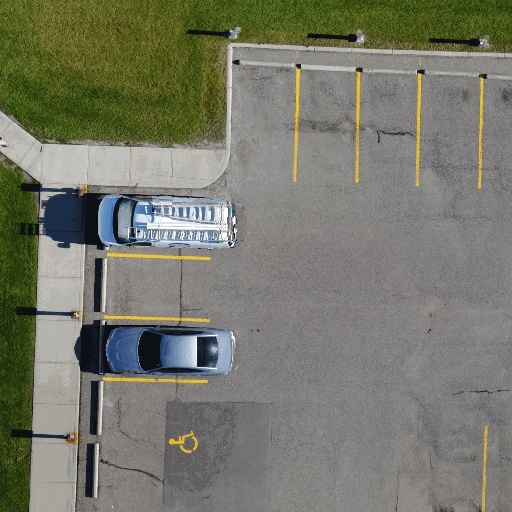
\includegraphics[width=3.8cm]{figures/Resized_Lot1.jpg}
\caption{Resized $512$ by $512$ parking lot image.}
\label{lot1}
\end{figure}

In the first experiment, we apply a fixed range yellow color filter defined 
in the HSV  space. 
Here, we take the lower bound of the yellow filter  to be
$(22, 60, 140)$ and the upper bound of the yellow filter  to be 
$(60,255,255)$. Shown as Figure \ref{lot1hsv}, with applying this color filter, 
we are able to keep only the yellow objects in the parking lot in the masked image. 
Following by Canny edge detection and Hough line transform, we can detect 
the yellow lines in the parking lot accurately (shown as panel $(c)$ of 
Figure \ref{lot1hsv}). However, a 
clear drawback for this approach is that we need to predefine 
a yellow filter in the HSV space, which can be hard to determine and have 
dependence according to the image. This motivates us to do the next 
trial, which applies color quantization to filter out the color 
other than yellow.

\begin{figure}[htp]
\centering
\begin{tabular}{ccc}
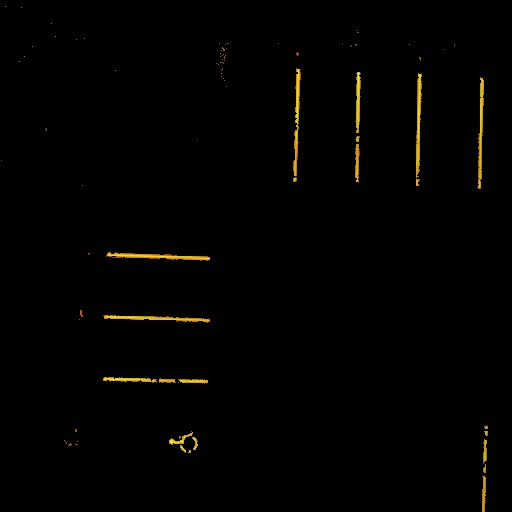
\includegraphics[width=3.8cm]{figures/Lot1mask.jpg}&
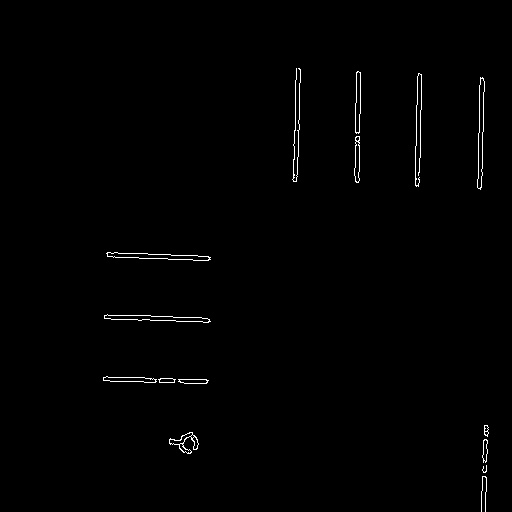
\includegraphics[width=3.8cm]{figures/Lot1edge.jpg}&
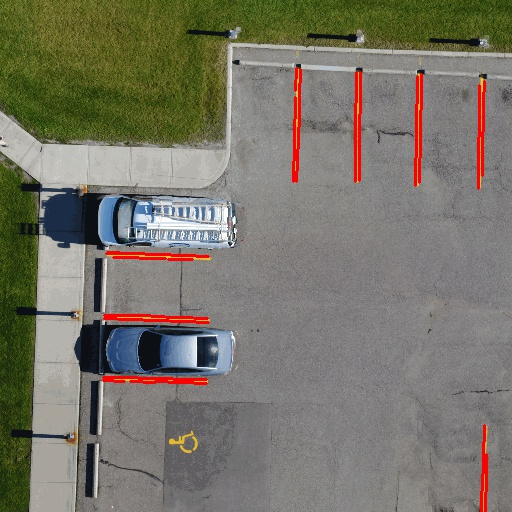
\includegraphics[width=3.8cm]{figures/Lot1detected.jpg}\\
$(a)$ & $(b)$ & $(c)$
\end{tabular}
\caption{Result for a fixed range yellow filter in HSV.
$(a)$ Color filtering result, 
$(b)$ Canny edge detection result,
$(c)$ Hough line detection result.}
\label{lot1hsv}
\end{figure}

In this experiment, we apply color quantization with $K$-means clustering of 
group $K=5$ in order to filter out the color other than yellow. 
The corresponding result is shown in Figure 
\ref{lot1k5}. In Figure $(a)$, we see that, in addition to the 
yellow lines in the parking lot, the sidewalk, cars and some other non-yellow
objects remain in the masked image. It leads to a noisy Canny edge detection
result as shown in panel $(b)$, so that we end up with a very inaccurate detection
of the yellow lines of the parking spots. It suggests us that $K=5$ may be too
small for the yellow color filtering, and a bigger number of $K$ should 
be applied 
in the clustering to see whether it can improve the result.

\begin{figure}[htp]\label{parking_lot_9}
\centering
\begin{tabular}{ccc}
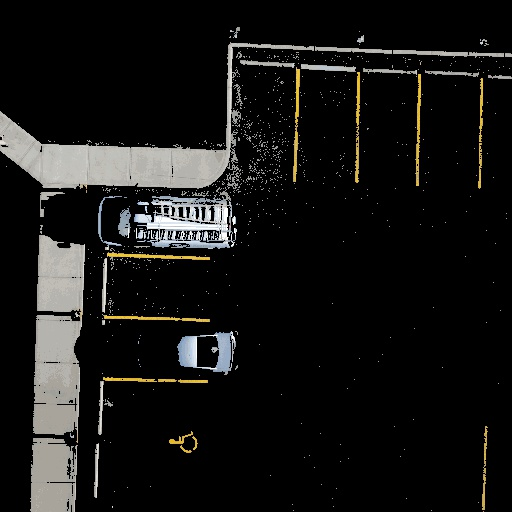
\includegraphics[width=3.8cm]{figures/Masked_Lot1k5.jpg}&
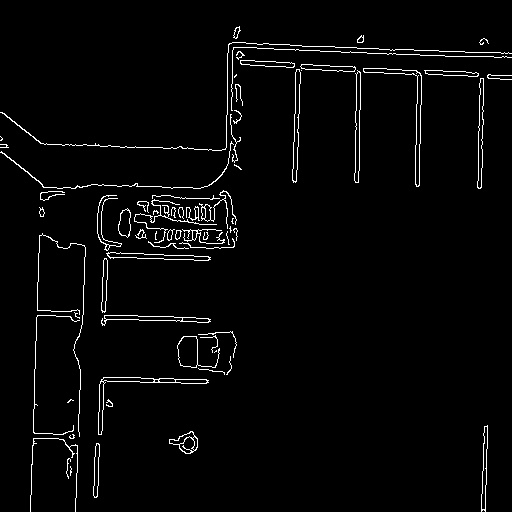
\includegraphics[width=3.8cm]{figures/Edge_Lot1k5.jpg}&
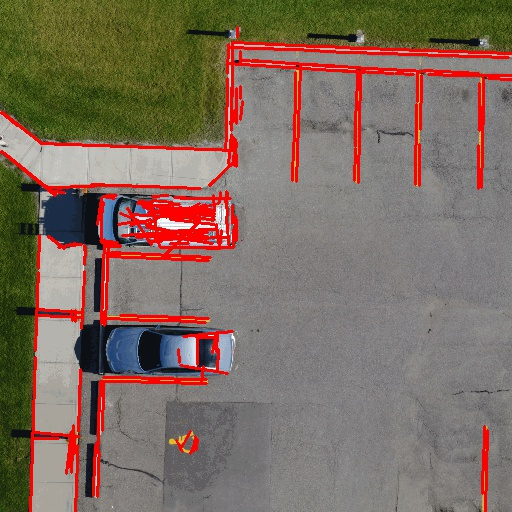
\includegraphics[width=3.8cm]{figures/Detected_Lot1k5.jpg}\\
$(a)$ & $(b)$ & $(c)$
\end{tabular}
\caption{Result for $K$-means with $K=5$. 
$(a)$ Color filtering result, 
$(b)$ Canny edge detection result,
$(c)$ Hough line detection result.}
\label{lot1k5}
\end{figure}

Finally, we present the result when either $ K=  6$ for $K$-means or
$5$ components for Gaussian mixture model is applied for the color 
quantization in Figure \ref{lot1result}. Here, for Gaussian mixture 
model,  we apply the ``tied" co-variance. 
Comparing the $K$-means with Gaussian mixture model, we see that, by applying 
either of the clustering method, yellow parking lines 
can be detected accurately. However, we have used one less
cluster group for Gaussian mixture model compared to $K$-means
in this example. 
After obtaining the edge detected image, we can then also apply 
the shape classification method (described in \S \ref{lineandbox}) to label
the yellow lines we are interested in with boxes. 


\begin{figure}[htp]
\centering
\begin{tabular}{cccc}
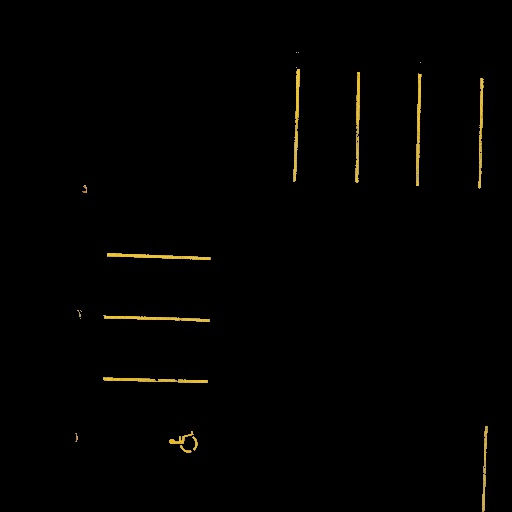
\includegraphics[width=3.5cm]{figures/Masked_Lot1.jpg}&
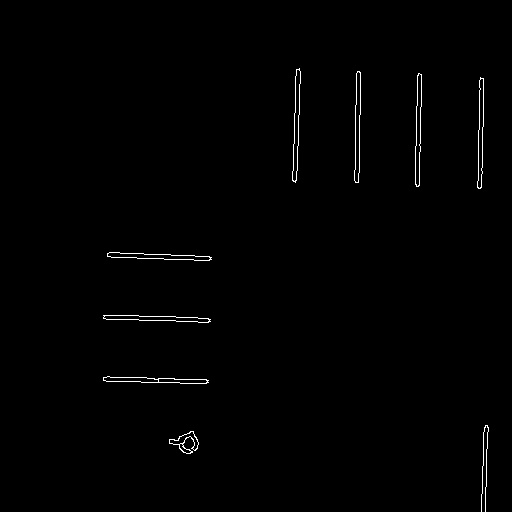
\includegraphics[width=3.5cm]{figures/Edge_Lot1.jpg}&
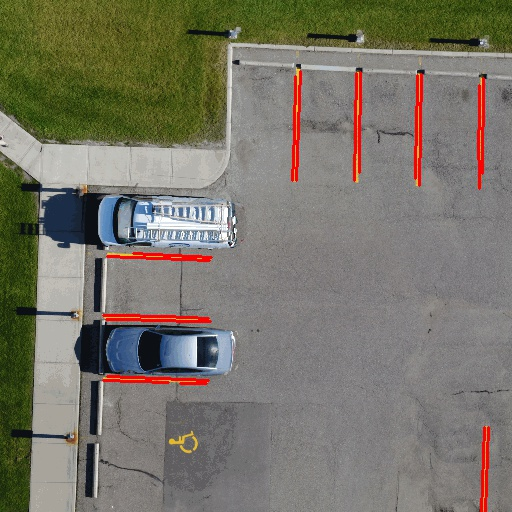
\includegraphics[width=3.5cm]{figures/Detected_Lot1.jpg}&
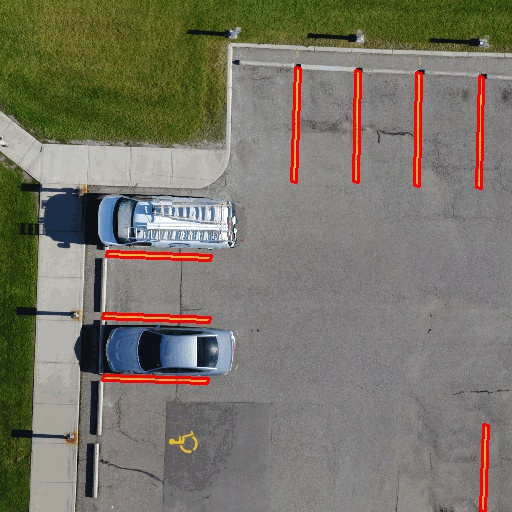
\includegraphics[width=3.5cm]{figures/Boxed_line_Lot1.jpg}\\
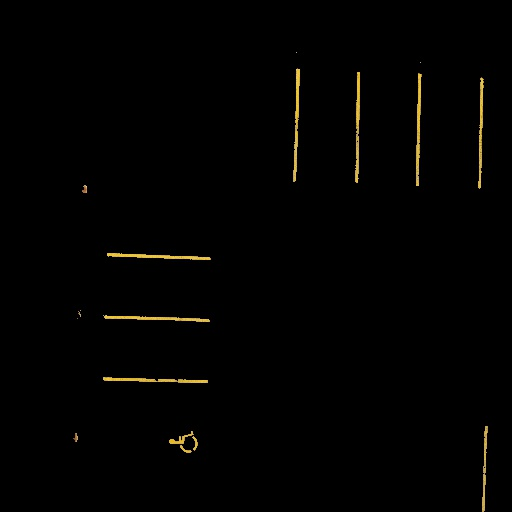
\includegraphics[width=3.5cm]{figures/Masked_Lot1G.jpg}&
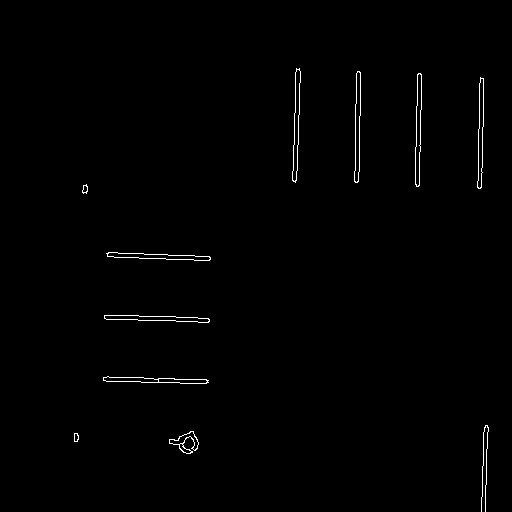
\includegraphics[width=3.5cm]{figures/Edge_Lot1G.jpg}&
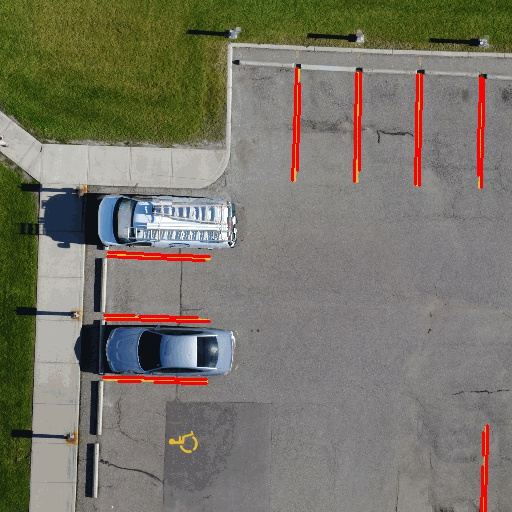
\includegraphics[width=3.5cm]{figures/Detected_Lot1G.jpg}&
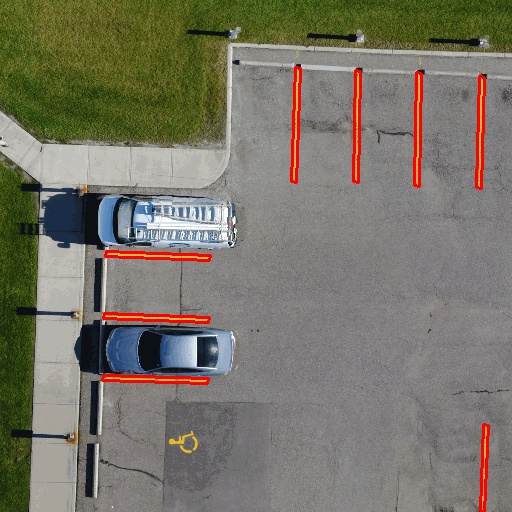
\includegraphics[width=3.5cm]{figures/Boxed_line_Lot1G.jpg}\\
$(a)$ & $(b)$ & $(c)$ & $(d)$
\end{tabular}
\caption{$(a)$ color filtering results, $(b)$ Canny edge detection results,
$(c)$ Hough line detection results, $(d)$ box labelling results. 
Results for $K$-means are shown on the top and for Gaussian mixture on the
bottom.}
\label{lot1result}
\end{figure}



\section{Conclusion and Future Work}

In this work, we use unsupervised machine learning methods and image processing techniques to identify yellow and white lines in aerial images of roads and parking lots. The general pipeline consists of the following sequential steps:

\begin{enumerate}
    \item Color quantization. Use unsupervised machine learning ($K$-means or Gaussian mixture models) to classify colors into clusters. The clustering can be applied to a number of images concatenated together, in which case a larger spectrum of colors is considered and the classifier can be saved for future use.
    \item Color filtering. Keep only yellow (white) pixels based on the color clusters. The output is a copy of the original image (or transformed color model) where all pixels not belonging to the cluster have been removed.  This step assumes that all yellow (white) pixels of interest are very similar. 
    \item Image smoothing. Apply a filter to eliminate isolated or faint pixels that remain after the color filter.
    \item Edge detection. Apply Canny edge detection to identify all enclosed regions that remain after color and smooth filters. The output is a binary image delimiting all filtered pixels.
    \item Contours. Identify the contour enclosing each of the group of pixels that has been edge detected. The output is a list of contour points delimiting each group of filtered pixels.
    \item Bounding boxes. Determine the minimal rectangle that encloses the contour. The output is a list of four (corner) points for each group of filtered pixels.
    \item Shape recognition. Use unsupervised machine learning (hierarchical clusters or $K$-means) or heuristic rules (aspect ratio larger than four) to classify and select those rectangles that are thin and long. The output is a subset of the bounding boxes.
    \item Labeling. Identify yellow (white) lines by plotting bounding boxes over the original image.
\end{enumerate}

We believe the pipeline above can be applied outside the data set that we considered. However, more experiments would be required with images including curved or angled road lines, etc.  From our experiments with the available data set, we identified a number of issues that we couldn't address due to time constrains. These issues and potential solutions/improvements are explained in the rest of this section.



\subsection{Future Work}

\subsubsection{Shadow}


Shadow is the main obstacle in this project. For example, from Figure \ref{lot11result} $(b)$ we can see the $K$-means clustering with Hough line detector cannot find all the yellow lines in the shadow area. This is because $K$-means can only pick up one yellow color while there is an obvious color difference between the normal yellow color in the bright area and dark yellow color in the shaded area. This can be partially solved by Gaussian Mixture model as shown in Figure \ref{lot11result} $(c)$, in which dark yellow color in shaded area is recognized as the normal yellow color in the bright area with a certain probability. However, we can see some yellow lines in shaded area are still missing from line detection.

\begin{figure}[htp]
\centering
\begin{tabular}{ccc}
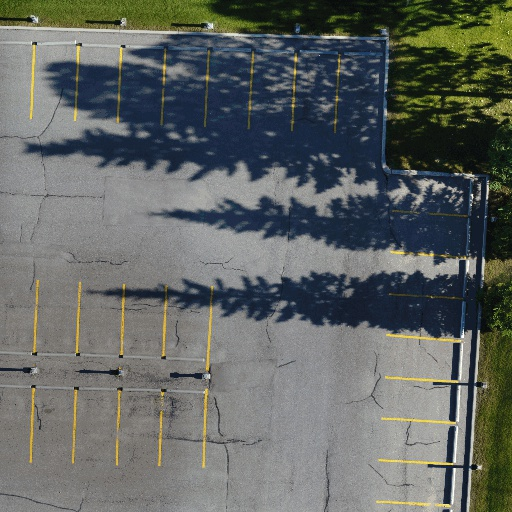
\includegraphics[width=3.8cm]{figures/Resized_Lot11.jpg}&
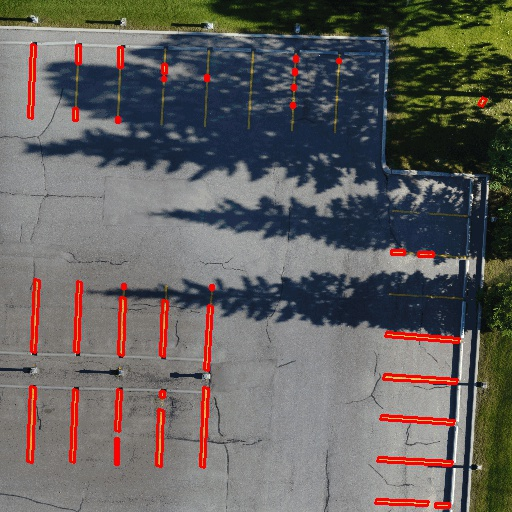
\includegraphics[width=3.8cm]{figures/Boxed_Lot11.jpg}&
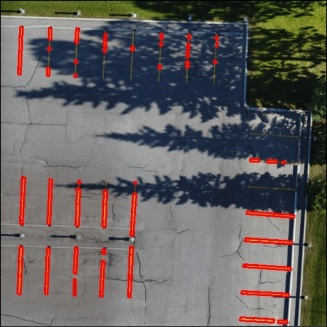
\includegraphics[width=3.8cm]{figures/detected_Lot11.jpg}\\
$(a)$ & $(b)$ & $(c)$
\end{tabular}
\caption{$(a)$ resized original image, $(b)$ $K$-means result,
$(c)$ Gaussian Mixture model result.}
\label{lot11result}
\end{figure}

One possible way to address the shadow issue is to modify the part of the image inside the shadow area while keeping the part of the image outside of the shadow unchanged. We got two different types of modifications, to increase the brightness of the shadow area by a certain value, or to modify the RGB color values of the shadow area and make them closer to the ones in the bright area. Both methods start with 
removing the texture of the image by mean shift filter. Then threshold the image and the shadow area can be picked up. Now change the color space of the shadow area from RGB to HSV so we can increase the brightness of the shaded area. (Or we can multiply the RGB color values of the shadow area to make the shadow area and the bright area have the same means of color values). Finally, we combine the images of the modified shadow area with the normal bright area to obtain the output. We can also use the mean shift filter again or inpainting tool to make the gap between the shadow area and bright area smoother. Figure \ref{lot11shadow} shows the result of brightening and color modification (the white spots inside shadow in panel $(c)$ come from small components removal after thresholding the original image, which is optional).

Another way to address with shadow parts is to apply the Homomorphic filter \cite{glasgio} to all images in the image process procedures, in order to improve the light exposure. This part is done before the color quantization. To be more specific, we first changed the color modes to HSV.
After that, we applied the Homomorphic filter on the low energy frequency on the brightness V channel, because the shadow part is related to the low energy frequency compared to the non-shadow parts. Then, we shifted the mean value of the V channel of the isomorphic filter images back to the original images.   We can see some results in Figure \ref{homo_transformed}. 

Together with other tools, one of the possible procedures to detect all lines in image with shadow is
\begin{enumerate}
    \item Shadow Modification
    \item Color Quantization
    \item Line Detection
\end{enumerate}
where we can change the order of the first two steps to compare the performance.


\begin{figure}[htp]
\centering
\begin{tabular}{ccc}
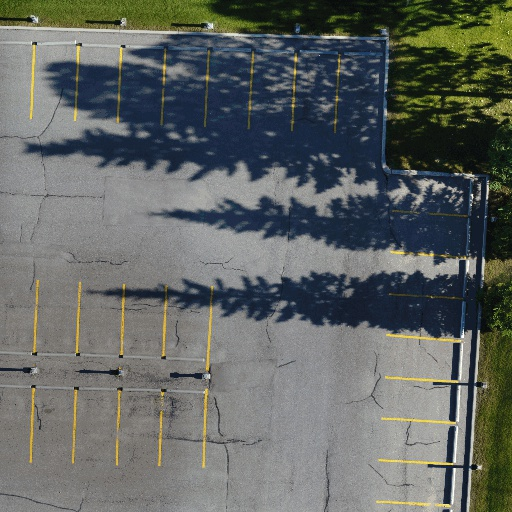
\includegraphics[height=3.6cm, width=3.9cm]{figures/Resized_Lot11.jpg}&
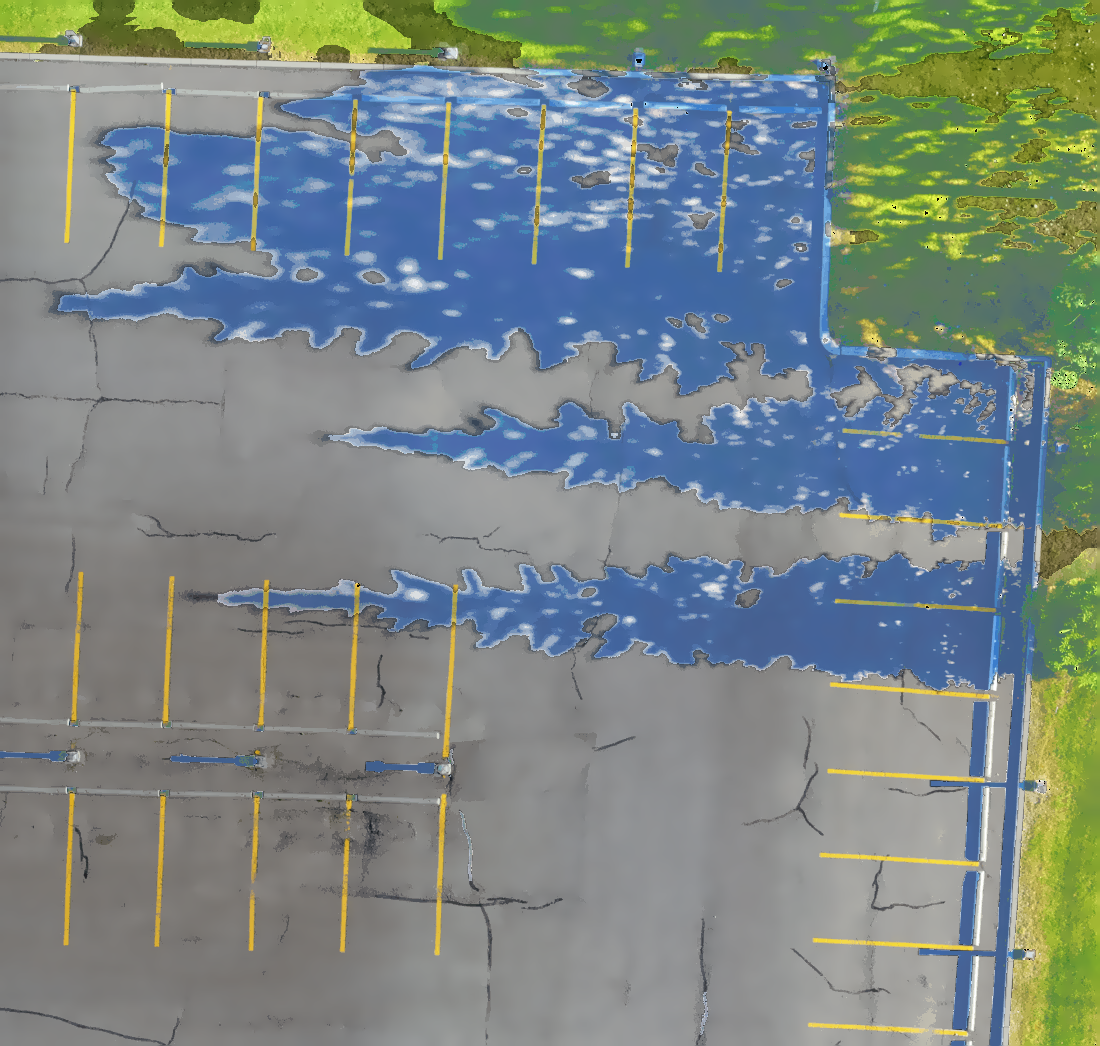
\includegraphics[width=3.8cm]{figures/Brightened Shadow.png}&
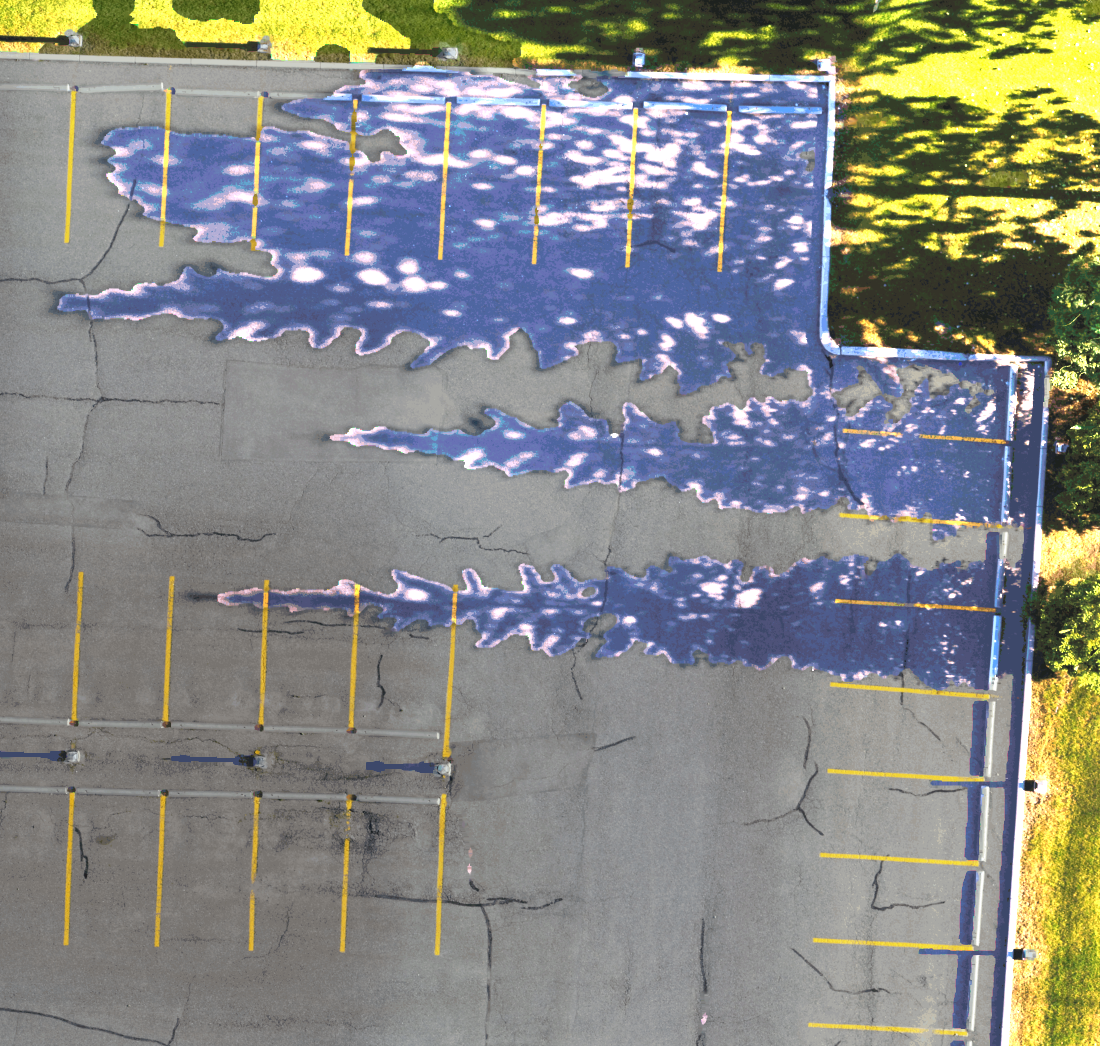
\includegraphics[width=3.8cm]{figures/Color Modified Shadow.png}\\
$(a)$ & $(b)$ & $(c)$
\end{tabular}
\caption{$(a)$ original image, $(b)$ brightened shadow, $(c)$ color modified shadow.}
\label{lot11shadow}
\end{figure}

\begin{figure}[htp]
\centering
\begin{tabular}{ccc}
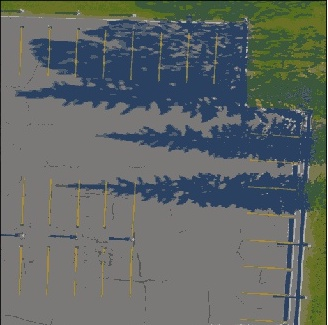
\includegraphics[width = 3.8cm]{figures/Transformed_Homomorphic_Lot11.jpg}&
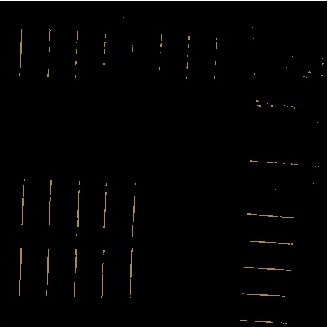
\includegraphics[width = 3.8cm]{figures/Masked_Homomorphic_Lot11.jpg}&
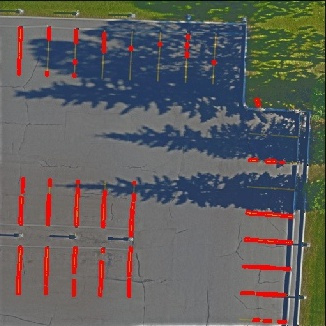
\includegraphics[width= 3.8cm]{figures/line_detected_Homomorphic_Lot11.jpg}\\
$(a)$ & $(b)$ & $(c)$
\end{tabular}
\caption{$(a)$ Homomorphic filtered image $(b)$ Color filtered image $(c)$ Line detection image with Homomorhpic filter}
\label{homo_transformed}
\end{figure}

\subsubsection{Unwanted White Lines}

When detecting white lines on roads, usually curbs are also detected at the same time. This creates problems if we want to distinguish white dash lines or marks in the middle of roads from curbs. As an example, Figure \ref{road3result} (b) shows curb affecting the detection of white dash lines if we only combine $K$-means clustering with Hough line detection.  Figure \ref{road3result} (c) shows if we apply one iteration of mean shift filter before $K$-means clustering, the influence of curbs becomes much smaller. 
It leaves us future work to do further investigation on how to properly apply 
mean shift filter to only detect the white dash lines in the middle of the road.

\begin{figure}[htp]
\centering
\begin{tabular}{ccc}
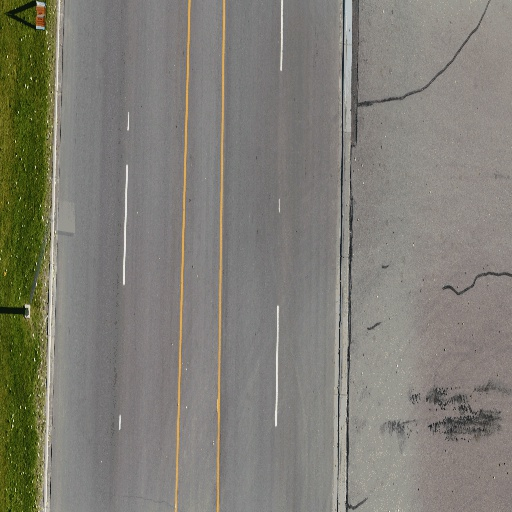
\includegraphics[width=3.8cm]{figures/Resized_Road3.jpg}&
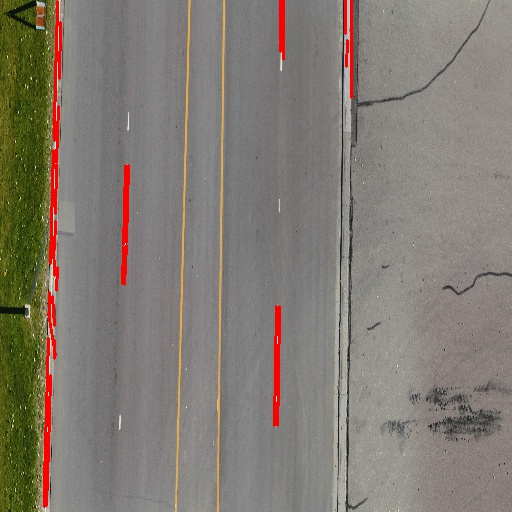
\includegraphics[width=3.8cm]{figures/Detected_Road3.jpg}&
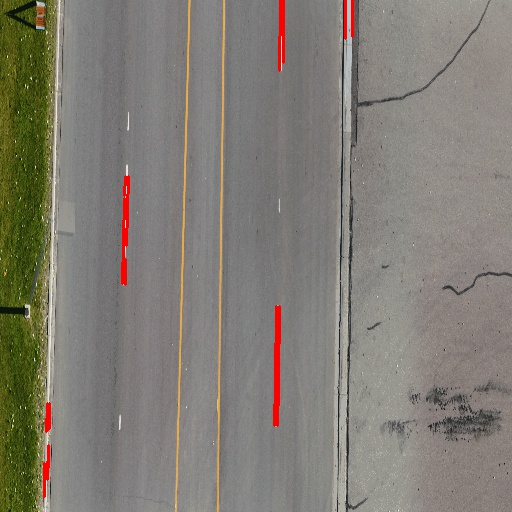
\includegraphics[width=3.8cm]{figures/Detected_Road3_meanshift.jpg}\\
$(a)$ & $(b)$ & $(c)$
\end{tabular}
\caption{$(a)$ original image, 
$(b)$ direct $K$-means result,
$(c)$ mean shift filtering before $K$-means result.}
\label{road3result}
\end{figure}

\subsubsection{Discontinued Lines}

Some images have discontinued lines due to washed out paint. In this case, two or more objects are identified which may be filtered out in the shape recognition step. We think that such lines can be reconstructed using machine learning based on complete lines present in the same image.

\subsubsection{Shape Recognition}

Currently, the shape recognition uses a fixed number of two clusters to classify lines from non-lines. However, this leads to sub-classifications of lines when there are only lines in the image, and misclassification of non-lines as lines when there are too many non-line objects in the image. We suggest using an unsupervised machine learning method with a variable number of clusters.


\subsubsection{Automated Parameter Selection}

Recall that the goal for this project is to create an automated 
recognition tool for road lines. When the color filtering step could be done 
automatically through machine learning techniques, we should not forget the fact 
that there are many parameters in this method which need to be pre-selected, 
such as the number of groups in clustering, the minVal, and MaxVal threshold 
in Canny edge detection, and three parameters in Hough line detection. 
Moreover, in the newly proposed shadow modification method shown as Figure 
\ref{lot11shadow} $(b)$, we also need to manually increase the HSV brightness 
value. Future work includes using machine learning to automate optimal parameter selection.



\section*{Acknowledgments}

We want to thank our industrial mentor Heather Vooys, Brian Bullas, Daniel McReynolds, the rest of the team at AERIUM Analytics, and our academic mentor Matthew Greenberg for their guidance, feedback, and support during the development of this project. We are also very grateful to Kristine Bauer, James Colliander, Ian Allison,  and the rest of the PIMS organizing committee and instructors of the Math$^{\text{Industry}}$ 2020 workshop.

\nocite{*}
\bibliographystyle{amsplain}
\bibliography{references}



\end{document}
